\documentclass{article}

\usepackage{amsmath,amssymb,geometry,minted,graphicx}
\usepackage{xepersian}

\setlength{\parindent}{0pt}
\setlength{\parskip}{3mm}

\newcounter{questionnumber}
\setcounter{questionnumber}{1}

\newcommand{\Q}{
\textbf{سوال \thequestionnumber)}
\stepcounter{questionnumber}
}

\newcommand{\py}[1]{
\begin{minted}{python}
#1
\end{minted}
}
\newcommand{\mat}[1]{
\begin{minted}{python}
#1
\end{minted}
}

\begin{document}
\LARGE
\begin{center}
\settextfont{IranNastaliq}

به نام زیبایی

%\begin{figure}[h]
%\centering
%\includegraphics[width=30mm]{kntu_logo.eps}
%\end{figure}

آموزش شبیه سازی درس احتمال مهندسی

\end{center}
\hrulefill
\large

در این آموزش، قصد داریم نمونه‌ی عملی یک شبیه سازی درس احتمال را پیاده سازی کنیم. فرض می شود که دانشجو، با دستورها و محیط کدنویسی متلب و پایتون آشنایی ابتدایی داشته باشد.

هدف: شبیه سازی پرتاب سکه

تعریف: میخواهیم پرتاب سکه‌ی سالمی را که با احتمال
$
\frac{1}{2}
$
رو یا پشت می‌آید، به تعداد
$
n
$
بار شبیه سازی کنیم. سپس، میانگین تعداد دفعاتی که سکه رو آمده است را در
$
n
$
بار پرتاب محاسبه کرده و بر حسب 
$
n
$
به ازای
$
1\le n\le 1000
$
رسم کنیم.

گام ها:

1) در متلب، یک اسکریپت جدید باز کنید.

1) در پایتون، یک اسکریپت جدید باز کرده و سپس، کتابخانه های numpy و matplotlib را به صورت زیر import کنید:

\begin{minted}{python}
import numpy as np
import matplotlib.pyplot as plt
\end{minted}

2) اکنون باید هر پرتاب سکه را شبیه سازی کنیم. از آنجا که در متلب و پایتون تولید عدد تصادفی با دستورهای خاصی امکان پذیر است، ابتدا قرارداد می‌کنیم که رو آمدن سکه را با $0$ و پشت آمدن را با $1$ نشان دهیم. در نتیجه، به تابعی نیاز داریم که اعداد $0$ و $1$ را یا احتمال یکسان برای ما تولید کند. این کار، به صورت زیر انجام می شود:

متلب: randi

\begin{minted}{matlab}
x=randi([0,1]);
disp(x)
\end{minted}

پایتون: np.random.randint

\begin{minted}{python}
import numpy as np
import matplotlib.pyplot as plt
x=np.random.randint(0,2)
print(x)
\end{minted}

3) اگر بخواهیم یک دنباله از اعداد تصادفی 0 و 1 تولید کنیم، به صورت زیر عمل می‌کنیم:

متلب:
\begin{minted}{matlab}
n=1000;
x=randi([0,1],1,n);
disp(x)
\end{minted}
پایتون:
\begin{minted}{python}
import numpy as np
import matplotlib.pyplot as plt
n=1000
x=np.random.randint(0,2,n)
print(x)
\end{minted}

4) حال باید $n$ را بین 1 تا 1000 تغییر داده،هر بار دنباله‌ای تصادفی از $n$ پرتاب سکه تولید کرده و تعداد دفعاتی که عدد $0$ رخ می‌دهد (سکه رو می‌آید) را بر $n$ تقسیم کنیم و به ازای هر $n$، نتیجه را در یک آرایه ذخیره کنیم:

متلب:
\begin{minted}{matlab}
tail_average=zeros(1,1000);

for n=1:1000
    coin_toss=randi([0,1],1,n);
    tail_average(n)=sum(coin_toss==0)/n;
end
\end{minted}
پایتون:
\begin{minted}{python}
tail_average=np.zeros(1000)

for n in range(1,1000+1):
    coin_toss=np.random.randint(0,2,n)
    tail_average[n-1]=sum(coin_toss==0)/n
\end{minted}

5) اکنون باید نتایج را چاپ کنیم. این کار را به صورت زیر انجام می‌دهیم:

متلب:
\begin{minted}{matlab}
plot(tail_average)
\end{minted}
پایتون:
\begin{minted}{python}
plt.plot(tail_average)
\end{minted}

((اختیاری)) می توان جهت افزایش خوانایی نمودارها، از عنوان روی محورهای افقی و عمودی یا بالای شکل و لجند بهره گرفت:

متلب:

\begin{latin}
\begin{minted}{matlab}
plot(tail_average)
title(['Average tail outcome vs. number',...
    ' of tosses in coin toss experiment'])
xlabel(`Number of tosses')
ylabel(`Average tail outcome')
\end{minted}
\end{latin}
پایتون:
\begin{latin}
\begin{minted}{python}
plt.plot(tail_average)
plt.title('Average tail outcome vs. number'+\
           ' of tosses in coin toss experiment')
plt.xlabel('Number of tosses')
plt.ylabel('Average tail outcome')
\end{minted}
\end{latin}

کد نهایی به صورت زیر است:

متلب:

\begin{latin}
\begin{minted}{matlab}
tail_average=zeros(1,1000);

for n=1:1000
    coin_toss=randi([0,1],1,n);
    tail_average(n)=sum(coin_toss==0)/n;
end

plot(1:1000,tail_average)

title(['Average tail outcome vs. number',...
    ' of tosses in coin toss experiment'])
xlabel('Number of tosses')
ylabel('Average tail outcome')
\end{minted}
\end{latin}
پایتون:
\begin{latin}
\begin{minted}{python}
import numpy as np
import matplotlib.pyplot as plt

tail_average=np.zeros(1000)

for n in range(1,1000+1):
    coin_toss=np.random.randint(0,2,n)
    tail_average[n-1]=sum(coin_toss==0)/n
    
plt.plot(tail_average)
plt.title('Average tail outcome vs. number'+\
           ' of tosses in coin toss experiment')
plt.xlabel('Number of tosses')
plt.ylabel('Average tail outcome')
\end{minted}
\end{latin}

و خروجی باید مشابه شکل زیر باشد:

\newpage

متلب:

\begin{figure}[h]
\centering
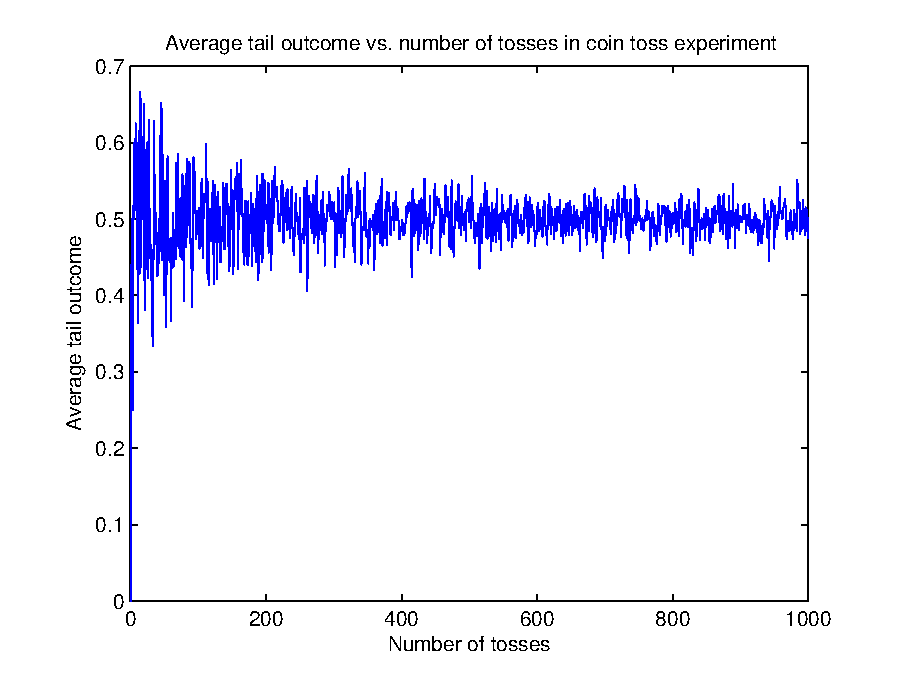
\includegraphics[width=100mm]{resultmat.eps}
\end{figure}

پایتون:
\begin{figure}[h]
\centering
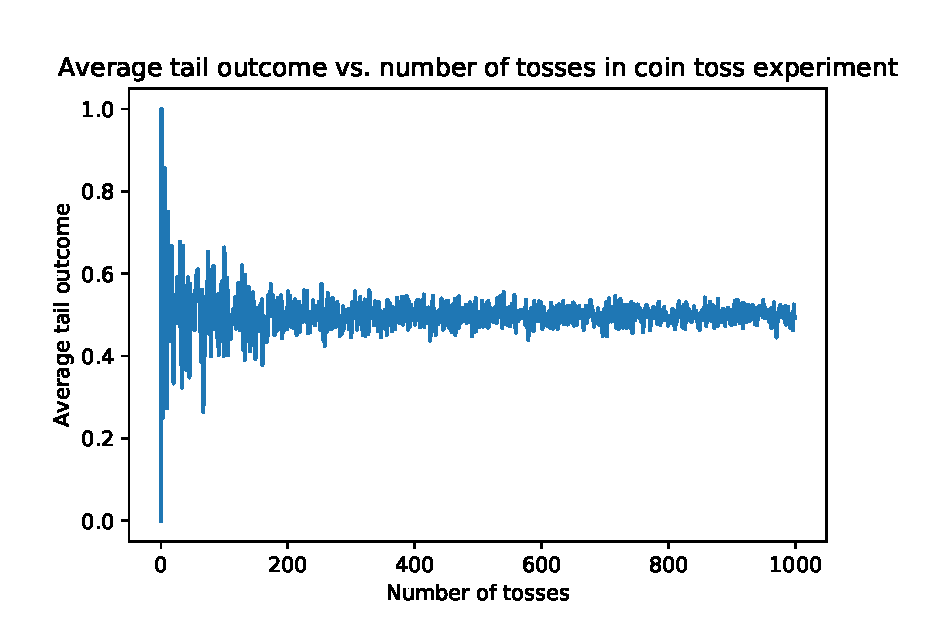
\includegraphics[width=100mm]{resultpy.eps}
\end{figure}






\end{document}
